\documentclass[10pt,journal]{IEEEtran}

\usepackage{graphicx}
\usepackage{cite}
\usepackage{amsmath}
\usepackage{tensor}
\usepackage{booktabs}

\DeclareMathOperator{\Tr}{Tr}
\DeclareMathOperator{\cov}{cov}

\begin{document}

\title{Smoothing and Interpolating Noisy GPS Data with Tension Splines}

\author{Jeffrey~J.~Early and Adam~M.~Sykulski%
\thanks{Jeffrey J. Early is with NorthWest Research Associates, 4118 148th Ave NE, Redmond, WA 98052, USA (email: jearly@nwra.com) } %
\thanks{Adam M. Sykulski is with the Data Science Institute and the Department of Mathematics and Statistics, Lancaster University, Bailrigg LA1 4YW, UK (email: a.sykulski@lancaster.ac.uk)}%
\thanks{Manuscript submitted February 29th, 2050.} }


\markboth{IEEE TRANSACTIONS ON SIGNAL PROCESSING}{}

\maketitle

\begin{abstract}
A technique is developed for smoothing and interpolating noisy GPS data using B-splines with tension. An interpolating B-spline basis set of arbitrary order is reformulated using knot placement, rather than the traditional approach of adding additional constraints on the coefficients. Adding tension to the interpolating spline to smooth noisy data is shown to be equivalent to a maximum likelihood problem on the velocity statistics of the underlying process. This insight allows for a nearly optimal choice of smoothing parameter, and shows the limitations of smoothing splines. Finally, we show how to modify the smoothing operator to account for the non-Gaussianity of GPS errors and reject outliers.


We show how the tension condition routinely employed in smoothing splines can be restated as a maximum likelihood problem and then how the tension parameter can be chosen based on physical reasoning. The GPS errors appear to be non-Gaussian, so we use a t-distribution in the maximum likelihood.
1. We reformulate the not-a-knot boundary condition in terms of spline placement, rather than additional conditions on the constrained problem.
2. We show how the tension condition routinely employed in smoothing splines can be restated as a maximum likelihood problem and then how the tension parameter can be nearly optimally chosen.
3. We show how to modify the smoothing operator to account for the non-Gaussianity of GPS errors and reject outliers.
\begin{itemize}
    \item degrees-of-freedom vs u scaling from knot paper is useful for initial estimate.
    \item confirm that dof/2 knot placement doesn't hurt anything
    \item new information occurs at roughly dt*dof.
    \item order of spline should \emph{not} continue the slope, but should be steeper. The reason is because this generates incoherent part of solution, which simply serves to add noise.
\end{itemize}
\end{abstract}

\begin{IEEEkeywords}
IEEE, IEEEtran, journal, \LaTeX, paper, template.
\end{IEEEkeywords}



%%%%%%%%%%%%%%%%%%%%%%%%%%%%%%%%%%%%%%%%%%%%%%%%%%%%%%%%%%%%%%%%%%%%%
% MAIN BODY OF PAPER
%%%%%%%%%%%%%%%%%%%%%%%%%%%%%%%%%%%%%%%%%%%%%%%%%%%%%%%%%%%%%%%%%%%%%

%%%%%%%%%%%%%%%%%%%%%%
%
\section{Introduction}
%
%%%%%%%%%%%%%%%%%%%%%%



In the summer of 2011 a series of dye-release experiments were conducted in the Sargasso Sea to assess the lateral diffusivity of oceanic processes \cite{shcherbina2015-bams}. Each of these experiments included an array of floating ocean surface buoys (drifters) drogued to the same depth as the dye and equipped with global positioning system (GPS) receivers recording locations every 30 minutes. Addressing the primary goal of understanding the physical processes controlling the lateral diffusivity requires significant processing of the drifter positions, including removing the uniform flow across all drifters, accounting for the large scale strain field, and finally analyzing the residual spectrum of the drifters for hints of a dynamical process. However, it quickly became clear that the GPS position data, which can have accurracies as low as a few meters \cite{faa2016-report}, was contaminated by outliers  with position jumps of hundreds of meters or more. Prior to analysis, the position data requires removing the outliers, and interpolating gaps to keep the position data synchronized in time across the drifter array.

The basic problem is ubiquitous: observations from GPS receivers return observed positions $x_i$ at times $t_i$ that differ from the true positions $x_{\textrm{true}}(t_i)$ by some noise $\epsilon_i \equiv x_i - x_{\textrm{true}}(t_i)$ with variance $\sigma^2$. The primary goal of \emph{smoothing} is to find the true position $x_{\textrm{true}}(t_i)$ not contaminated by the noise, while the primary goal of \emph{interpolating} is to find the true position $x_{\textrm{true}}(t)$ between observation times.

The approach taken here is to use smoothing splines. Our model for the `true' path $x(t)$ is specified using interpolating b-splines $X^K(t)$ such that,
\begin{equation}
\label{b-spline-model-intro}
    x(t) = \sum_{i=1}^N \xi^i X^K_i(t)
\end{equation}
where $K$ is the order (degree $S=K-1$) of the spline. For $N$ observations we construct $N$ b-splines such that $x(t_i)=x_i$ for appropriately chosen coefficients $\xi_i$. In order to smooth the data we choose coefficients $\xi_i$ that minimize the penalty function,
\begin{equation}
\label{smoothing-spline}
\phi =  \frac{1}{N}\sum_{i=1}^{N} \left( \frac{x_i - x(t_i)}{\sigma} \right) ^2 + \lambda_T \int_{t_1}^{t_N} \left(\frac{d^T x}{dt^T}\right)^2 \, dt
\end{equation}
for some tension parameter $\lambda_T$. If $\lambda_T \rightarrow 0$ then $\phi=0$ because $x(t_i)=x_i$, but if $\lambda_T \rightarrow \infty$ then this forces the $x(t)$ to an $T$-th order polynomial (e.g., when $T=2$, the model is forced to be a straight line because it has no second derivative). The resulting path $x(t)$ is known as a smoothing spline and was first introduced in modern form by \cite{reinsch1967-nm}, but according to \cite{deboor1978-book} the idea dates back to \cite{whittaker1923-pems}. Once $S$ and $T$ are chosen, the smoothing spline has one free parameter ($\lambda_T$) and its optimal value can be found by minimizing the expected mean square error when the variance of the noise is known \cite{craven1979-nm}.

As a practical matter there are three issues that still need to be addressed before smoothing splines can be applied to the drifter data:
\begin{enumerate}
    \item how do we choose $S$ and $T$---and how do these choices affect the recovered power spectrum?
    \item how do we modify the spline fit to accommodate the non-Gaussian errors of GPS receivers?
    \item how do we identify and remove outliers?
\end{enumerate}
To address these issues, but also serve as a practical guide to other practitioners, we start by reviewing B-splines in section \ref{sec:interpolation} and introduce the canonical interpolating spline that is used as the underlying model for path $x(t)$ (equation \ref{b-spline-model-intro}) throughout this manuscript. Section \ref{sec:smoothing_spline} takes a broad look at tension splines and the assumptions they make on the underlying physical process. We show that the tension parameter $\lambda_T$ scales with the degrees-of-freedom and root-mean-square value of the tensioned derivative, suggesting that it can be estimated without minimizing the mean-square error. We also show that the penalty function in equation \ref{smoothing-spline} can be formulated as a maximum likelihood problem and that applying tension is equivalent to assuming a Gaussian distribution on the tensioned derivative of the underlying process.

Section \ref{sec:spline_order_tension_order_spectrum} uses synthetic data to test a number of choices that have to be made. We first establish that setting $T=S$ is optimal. We then show that the tension parameter can be chosen \emph{a priori} (without optimization of the mean-square error) when the number of degrees-of-freedom can be estimated from the data. This estimate for the degrees-of-freedom can then be used to reduce the coefficients, $\xi^i$, in the splines fit without sacrificing mean-square-error. Finally, we show the effect of different choices of $S$ on the resulting power spectrum and show how the degrees-of-freedom in the fit can be used to establish the highest resolved frequency.

The second half of the manuscript addresses issues specific to GPS positions errors. In section \ref{sec:drifter_data_set} we show that the GPS errors are not Gaussian distributed, but t-distributed and show how to modify the technique for a t-distribution. In section \ref{sec:outliers} we show how outliers can be removed from the dataset before fitting with a tension spline.



% Given the ubiquity of this basic problem, there are certainly many approaches to finding the true path $x(t)$---the approach taken here is to use maximum likelihood. The central idea of maximum likelihood is to ask ``Given a particular path $x(t)$, what is the probability that this dataset $(t_i,x_i)$ could have occurred?'' \cite{press1992-book}. The goal is then to find the path that is most likely to have produced that dataset.

% Conceptually there are two major pieces needed to solve this problem,
% \begin{enumerate}
% \item we need to specify the form of the path---a model, and
% \item we need to specify at least one probability distribution function (PDF) for some aspect of the signal or errors.
% \end{enumerate}

% The approach taken in this manuscript is to specify the model using smoothing splines. In section \ref{sec:interpolation} we review b-splines and introduce the canonical interpolating spline that is used as the underlying model for path $x(t)$ throughout this manuscript. Section \ref{sec:smoothing_spline} formulates the maximum likelihood problem in terms of the error in positions and the velocity of the particle. This is shown to be equivalent to using a tensioned smoothing spline. Section \ref{sec:optimal_parameter} shows how the optimal tension parameter can be chosen directly from the data time series.


%%%%%%%%%%%%%%%%%%%%%%
%
\section{Interpolating Spline}
\label{sec:interpolation}
%
%%%%%%%%%%%%%%%%%%%%%%

\begin{figure*}[h]
  \centerline{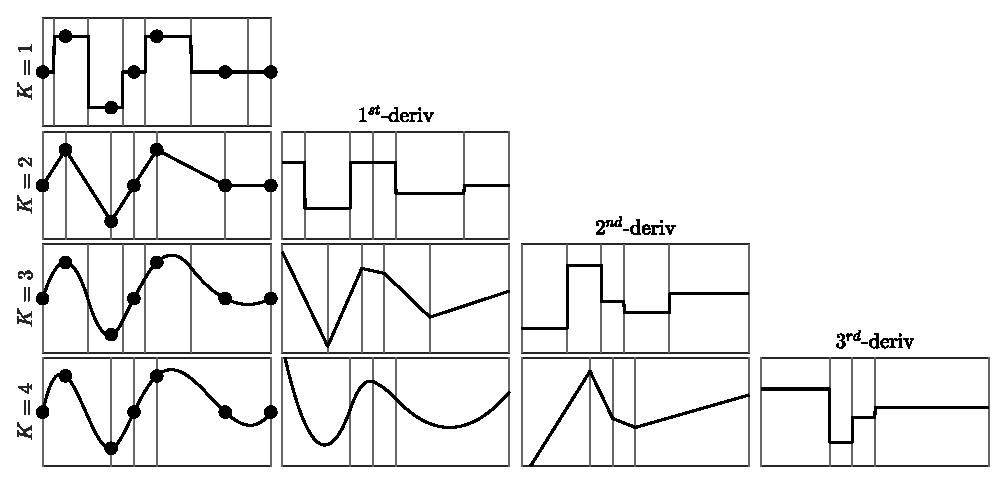
\includegraphics[width=39pc,angle=0]{figures/interpolation}}
  
  \caption{This shows an example of interpolating between 7 data points. The data points are shown as circles, and the interpolated function is shown as a solid black lines. We show four different orders of interpolation $K=1..4$ (rows) and their nonzero derivatives (columns). The thin vertical grey lines are the knot points.}
  \label{interpolation}
\end{figure*}

Assume that we are given $N$ observations of a particle position $(t_i,x_i)$ with no errors. The simplest possible form of interpolation would be a nearest neighbor method that assigns the position of the particle to the nearest observations in time. The resulting interpolated function $x(t)$ is a polynomial of \emph{order} $K=1$ (piecewise constant), shown in the top row of figure \ref{interpolation}. The next level of sophistication is to assume a constant velocity between any two observations and use that to interpolate positions between observations, second row of figure \ref{interpolation}. This also means that we now have a piecewise constant function $\frac{dx}{dt}$ that represents the velocity of the particle, shown in the second row, second column of figure  \ref{interpolation}. This is a polynomial function of order $K=2$.

It is slightly less obvious how to proceed to a polynomial of order $K=3$. With $N$ data points we can construct a piecewise constant acceleration (the second derivative) using the $N-2$ independent accelerations, but where to place $\emph{knot points}$ that define the boundaries of the regions and how to maintain continuity is slightly less clear. The approach taken here is to use B-splines.

%%%%%%%%%%%%%%%%%%%%%%
\subsection{B-Splines}
%%%%%%%%%%%%%%%%%%%%%%

A B-spline (or basis spline) of \emph{order} $K$ (\emph{degree} $S=K-1$) is a piecewise polynomial that maintains nonzero continuity across $S$ knot points. The knot points are a nondecreasing collection of points in time that we will denote with $\tau_i$. The basic theory is well documented in \cite{deboor1978-book}, but here we will present a reduced version specifically tailored to our needs.

The $m$-th B-spline of order $K=1$ is defined as,
\begin{equation}
X^1_m(t) \equiv \begin{cases}
1      & \text{if $ \tau_m \leq t < \tau_{m+1}$}, \\
0     & \text{otherwise}.
\end{cases}
\end{equation}
This is the rectangle function as shown in the first row, first column of figure \ref{bsplines}. If we are given $P$ knot points, then we can construct $P-1$ B-splines of order $K=1$, although notice that if a knot point is repeated this will result in a spline that is zero everywhere. To represent an interpolating function $x(t)$ for the $N$ observations of a particle position $(t_i,x_i)$ we define $N+1$ knot points as,
\begin{equation}
\tau_m = \begin{cases}
t_1      & \text{$m=1$}, \\
t_{m-1} + \frac{t_m-t_{m-1}}{2}	  & \text{$1<m \leq N$}\\
t_N     & \text{$m>N$}.
\end{cases}
\end{equation}
This will create $N$ independent basis functions that provide support for the region $t_1 \leq t \leq t_N$ (provided the last spline is defined to include the last knot point). The interpolating function $x(t)$ is defined as $x(t) \equiv  X^1_m(t) \xi^m$ where the coefficients $\xi^m$ are found by solving $X^1_m(t^i) \xi^m = x^i$. The result of this process is shown in figure \ref{interpolation} for 7 irregularly spaced data points.

All higher order B-splines are defined by recursion,
\begin{equation}
X^K_m(t) \equiv \frac{t - t_m}{t_{m+K-1} - t_m} X^{K-1}_m(t) + \frac{t_{m+K}-t}{t_{m+K} - t_{m+1}} X^{K-1}_{m+1}(t).
\end{equation}
This recursion formula takes two neighboring lower order splines and ramps the left one up over its nonzero domain and ramps the right one down over its nonzero domain. The result of this process is to create splines that span across one additional knot point at each order, and maintain continuity across one more derivative. Examples are shown in figure \ref{bsplines}.

Any knot points that are repeated $T$ times will result in a total of $T-1$ splines of order one that are everywhere zero. This has the effect of introducing discontinuities in the derivatives for higher order splines. For our purposes, we will only use this feature to prevent higher order splines from crossing the boundaries. For $K=2$ order splines we will use $N+2$ knot points at locations,
\begin{equation}
\tau_m = \begin{cases}
t_1      	& \text{$m \leq 2$}, \\
t_{m-1}	& \text{$2 < m \leq N$}\\
t_N 		& \text{$m > N$}.
\end{cases}
\end{equation}
This creates a knot point at every observation point, but repeats the first and last knot point. This has the effect of terminating the first and last spline at the boundary and creating $N$ second order B-splines, $X^2_m(t)$. Once again the interpolating function $x(t)$ is defined as $x(t) \equiv  X^2_m(t) \xi^m$ where the coefficients $\xi^m$ are found by solving $X^2_m(t^i) \xi^m = x^i$. The second row of figure \ref{interpolation} shows an example.

This process can be continued to higher and higher order B-splines. For splines that are of \emph{even} order, we create $N+K$ knots points with
\begin{equation}
\tau_m^{\text{$K$-even}} = \begin{cases}
t_1      	& \text{$m \leq K$}, \\
t_{m-K/2}	& \text{$K < m \leq N$}\\
t_N 		& \text{$m > N$}
\end{cases}
\label{even-knots}
\end{equation}
and for splines that are \emph{odd} order, we create $N+K$ knot points with,
\begin{equation}
\tau_m^{\text{$K$-odd}} = \begin{cases}
t_1      	& \text{$m \leq K$}, \\
t_{m-\frac{K+1}{2}} + \frac{t_{m+1-\frac{K+1}{2}}-t_{m-\frac{K+1}{2}}}{2}	& \text{$K < m \leq N$}\\
t_N 		& \text{$m > N$}
\end{cases}
\label{odd-knots}
\end{equation}
The knot points are chosen specifically to create $N$ splines for the $N$ data points such that the interpolated function $x(t)$ crosses all $N$ observations $(t_i,x_i)$. The path $x(t)$ is the \emph{canonical interpolating spline of order K}. Examples are shown in figure \ref{interpolation}.

\begin{figure}
  \centerline{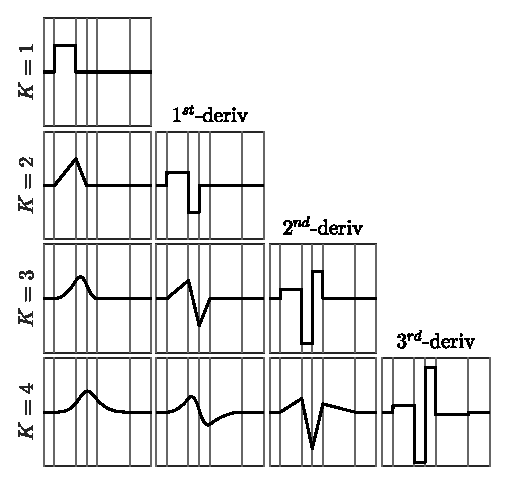
\includegraphics[width=19pc,angle=0]{figures/bsplines}}
  \caption{This shows an example B-spline and its derivatives (columns) for orders $K=1..4$ (rows).}
  \label{bsplines}
\end{figure}

The knot placements in equations \ref{even-knots} and \ref{odd-knots} are equivalent to the \textit{not-a-knot} boundary conditions described in \cite{deboor1978-book} and used in the cubic spline implementation in \texttt{Matlab}. In the usual formulation of the not-a-knot boundary condition, the knot positions do not change as a function of spline order, and therefore additional constraints have to be added at each order---especially the requirement that the highest derivative maintain continuity near the boundaries. In the formulation here, these constraints are implicit in equations \ref{even-knots} and \ref{odd-knots}.

It appears to be true that this formulation results in a spline with highest derivative equivalent to the lowest order finite difference for that derivative.

The examples shown here are implemented with a series of classes in Matlab. The Matlab class \texttt{BSpline} creates and evaluates a complete B-Spline basis set given a set of knot points. Its subclass \texttt{InterpolatingSpline} creates an interpolating splines of arbitrary order given a set of data points $(t_i, x_i)$, essentially generalizing the cubic spline implementation that ships with Matlab.

%%%%%%%%%%%%%%%%%%%%%%
\subsection{Synthetic Data}
\label{sec:synthetic_data}
%%%%%%%%%%%%%%%%%%%%%%

Throughout this manuscript we generate synthetic data for both the signal and the noise. The velocity of the signal is generated from a Gaussian process known as the Mat\'ern \cite{lilly2017-npg}. The spectrum of the Mat\'ern is given by
\begin{equation}
S(\omega) = \frac{A^2}{(\omega^2 + \lambda^2)^{p/2}}
\end{equation}
with $p>1$ which has finite amplitude at low frequencies and power-law fall off at high frequencies, two physically realistic properties observed, among other things, in ocean surface drifters \cite{sykulski2016-jrssc}.

%The Mat\'ern is a Gaussian process, which is important for the discussion in section \ref{sec:maximum_likelihood}.

For these experiments we choose values of $p=2,3,4$ so that the high frequency spectrum is proportional to $\omega^{-2}$, $\omega^{-3}$, $\omega^{-4}$. The Mat\'ern is used to generate the \emph{velocity} of the signal and integrated to get the positions. Parameters are chosen such that the square root of velocity variance in each direction is $u_{\textrm{rms}}=0.20$ m/s and the damping scale $\lambda^{-1}=30$ minutes. These choices somewhat resemble the data from the drifters. Figure \ref{varied_slope} shows an example velocity spectrum of the signal with $\omega^{-2}$.

The position data is contaminated with (white) Gaussian noise with $\sigma=10$ meters, a value chosen to resemble GPS errors. In section \ref{gps_position_errors} we consider consider noise generated from a Student's t-distribution which more accurately reflects the GPS errors.

For all of these experiments we use a range of \emph{strides}, that is, subsampled versions of the underlying process as input into the spline fits. A stride of 100 indicates that the signal is subsampled to 1 every 100 data points. This lets us evaluate the quality of fit against different sampling rates.

%%%%%%%%%%%%%%%%%%%%%%
\subsection{Spline degree, $S$} \label{spline_degree}
%%%%%%%%%%%%%%%%%%%%%%

\begin{figure}
  \centerline{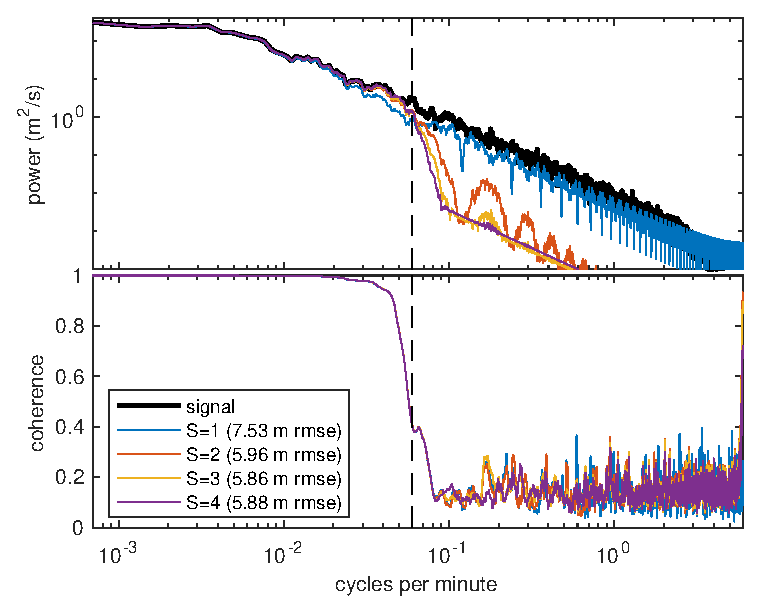
\includegraphics[width=19pc,angle=0]{figures/interpolation_spectrum_slope2degreeVaried}}
  
  \caption{The upper panel shows the velocity spectrum of the signal (black). The blue, red, and orange lines show the spectrum of the interpolating spline fit to the data with a stride of 100 for $S=1$, $S=2$, and $S=3$, respectively. The dashed vertical line denotes the Nyquist frequency of the strided data. The bottom panel shows the coherence between the smoothed signals and the true signal.}
  \label{varied_slope}
\end{figure}

We first examine a synthetic signal \emph{uncontaminated} by noise, to examine the role of spline degree, $S$, on the interpolated fit. As noted in \cite{craven1979-nm}, the degree of the spline sets its roughness. In terms of the power spectrum, this corresponds to the high frequency slope as can be seen in figure \ref{varied_slope} which shows fits with $S=1$, $S=2$, and $S=3$. Setting $S=1$ produces a high frequency fall off in the spline fit of $\omega^{-2}$. Although this would appear to be a desirable feature when fitting to a process with slope $\omega^{-2}$, the mean square error is consistently higher.

The bottom panel of figure \ref{varied_slope} shows the coherence between the spline fit and the true signal. There is no discernible difference in coherence between spline fits with $S=1$, $S=2$, and $S=3$. The coherence quickly drops to near zero at the same frequency in all three cases. The implication here is that the spline fits are essentially producing noise at frequencies above the loss-of-coherence. This is why the shallower slopes (with more variance at high, incoherent frequencies) have a larger mean square error than the steeper slopes (with less variance at high, incoherent frequencies). The conclusion here is that smoother is better: it's better to use an unnecessarily high order spline

As an aside, in an earlier version of this manuscript we test 

%%%%%%%%%%%%%%%%%%%%%%
%
\section{Smoothing Spline}
\label{sec:smoothing_spline}
%
%%%%%%%%%%%%%%%%%%%%%%

A typical starting point for maximum likelihood is to establish the probability distribution function (PDF) of the errors, $\epsilon_i \equiv x_i - x_{\textrm{true}}(t_i)$. The canonical example in one-dimension (e.g., \cite{press1992-book}) is to assume that the error in our position measurements are Gaussian i.i.d. and are therefore drawn from the following probability distribution
\begin{equation}
\label{gaussian_pdf}
p_g(\epsilon|\sigma_g) = \frac{e^{-\frac{1}{2}\frac{\epsilon^2}{\sigma_g^2}} }{\sigma_g \sqrt{ 2 \pi}}
\end{equation}
where $\sigma_g$ is the standard deviation. This assumption alone places no assumptions on the signal itself, only on the structure of the noise.

The probability of the observed data given some model $x(t)$ is,
\begin{equation}
\label{max-gaussian}
P = \frac{1}{\sigma \sqrt{2 \pi}} \prod_{i=1}^{N}  \exp \left[ -\frac{1}{2} \left( \frac{x_i - x(t_i)}{\sigma} \right)^2 \right]
\end{equation}
where we've taken $\sigma=\sigma_g$.

Maximizing the probability function in equation \ref{max-gaussian} is also the same as minimizing its argument---up to a constant this is the log likelihood, called the penalty function,
\begin{equation}
\label{least-squares}
\phi = \frac{1}{N}\sum_{i=1}^{N} \left( \frac{x_i - x(t_i)}{\sigma} \right)^2 .
\end{equation}
Stated in this way it is plain to see that this is the same as asking for the `least-squares' fit of the errors.


%%%%%%%%%%%%%%%%%%%%%%
\subsection{Smoothing spline penalty function}
%%%%%%%%%%%%%%%%%%%%%%

The model used here will be the canonical interpolating spline of order $K$ described in section \ref{sec:interpolation}. Of course, we've chosen our knot points such that the model intersects each observations and this certainly maximizes equation \ref{max-gaussian} (and minimizes equation \ref{least-squares}) because all the errors are zero, but the resulting distribution of errors (a delta function at zero) doesn't look anything like the assumed Gaussian distribution. Thus, if we want the error distribution that we get out to look like that which we assumed, it is also necessary to \emph{constrain} the problem in some way.

The smoothing spline augments the penalty function of equation \ref{least-squares} by adding a global constraint on the $m$-th derivative of the resulting function,
\begin{equation*}
\tag{\ref{smoothing-spline} revisited}
\phi =  \frac{1}{N}\sum_{i=1}^{N} \left( \frac{x_i - x(t_i)}{\sigma} \right) ^2 + \lambda_T \int_{t_1}^{t_N} \left(\frac{d^T x}{dt^T}\right)^2 \, dt.
\end{equation*}
If $\lambda_T \rightarrow 0$ then this reduces to the least-squares fit in equation \ref{least-squares}, but if $\lambda_T \rightarrow \infty$ then this forces the model to an $T$-th order polynomial (e.g., when $T=2$, the model is forced to be a straight line because it has no second derivative).

The first term of equation \ref{smoothing-spline} is proportional to the sample variance,
\begin{equation}
\label{sample_variance}
\hat{\sigma}^2  \equiv \frac{1}{N} \sum_{i=1}^{N} \left( x_i - x(t_i) \right) ^2,
\end{equation}
which is expected to scale like
\begin{equation}
\label{sample_variance_variance}
\hat{\sigma}^2 = \frac{n_{\textrm{eff}}-1}{n_{\textrm{eff}}} \sigma^2
\end{equation}
where $n_{\textrm{eff}}$ is effective sample size. For a large number of sample size the sample variance matches the true variance, but as will be discussed in section \ref{sec:spline_order_tension_order_spectrum} this distinction is key to optimal parameter choice.

There is a very simple physical interpretation for the second term in equation \ref{smoothing-spline}. Consider the case where $T=1$ so that the smoothing spline is a constraint on velocity. When averaged over the integration time, the integral produces the root mean square velocity, $u_{\textrm{rms}}$, which means that the second term scales like $u_{\textrm{rms}}^2 (t_N-t_1)$. In general, where $x^{(T)}_{\textrm{rms}}$ is the root-mean-square of the $T$-th derivative, this means that
\begin{equation}
\label{lambda}
\lambda_T = \frac{n_{\textrm{eff}}-1}{n_{\textrm{eff}}} \frac{1}{ \left(x^{(T)}_{\textrm{rms}}\right)^2 (t_N-t_1)}.
\end{equation}
The interpretation of the smoothing spline is therefore that the two terms are balanced by a relative weighting of the sample variance and mean-square of the $T$-th derivative of the physical process.

%%%%%%%%%%%%%%%%%%%%%%
\subsection{Smoothing spline maximum likelihood}
\label{sec:maximum_likelihood}
%%%%%%%%%%%%%%%%%%%%%%

The penalty function for the smoothing spline (\ref{smoothing-spline}) can be restated in terms of maximum likelihood under some conditions (see chapter 3.8 in \cite{green1994-book}). Assume that in addition to knowing about how the measurement errors are distributed like in equation \ref{max-gaussian}, that we also know how the velocity of underlying physical process is distributed. For example, in geophysical turbulence it has been shown that the velocity probability distribution function is like the Laplace distribution \cite{bracco2000-pf}. To recover the smoothing spline, we need to consider the case where the velocity PDF is Gaussian. Stated as maximum likelihood, this means that at \emph{any given instant} (not just the times of observation) we expected the model velocity to look Gaussian. We can discretize the problem by sampling the velocity $Q$ at times $t_q = t_1 + q \Delta t_q$ where $\Delta t_q=\frac{t_N-t_1}{Q-1}$ and $q=0..Q-1$. The maximum likelihood is thus stated as,
\begin{equation}
\label{gaussian-max-likelihood}
\begin{split}
P =   \prod^N _{i=1}\frac{1}{\sigma \sqrt{2 \pi}}\exp \left[ -\frac{1}{2} \left( \frac{x_i - x(t_i)}{\sigma} \right)^2 \right] \\ \nonumber \cdot  \prod^{Q}_{q=1}\frac{\sqrt{\alpha}}{x^{(T)}_{\textrm{rms}} \sqrt{2 \pi}} \exp \left[  - \frac{\alpha}{2} \left(  \frac{x^{(T)}(t_q)}{x^{(T)}_{\textrm{rms}}} \right)^2 \right]
\end{split}
\end{equation}
which is simply the joint probability of the error distribution from equation \ref{max-gaussian} and the velocity distribution of the underlying physical process. We also include parameter $\alpha$ for convenience in order to set the relative weighting between the two distributions, although it could be absorbed into the definition of $x^{(T)}_{\textrm{rms}}$. Writing equation \ref{gaussian-max-likelihood} as a penalty function (after converting the product of exponentials into exponentials of sums), we have that
\begin{align}
\label{smoothing-spline-log-likelihood}
-\log(P)=& \frac{1}{2}\sum^N _{i=1}  \left( \frac{x_i - x(t_i)}{\sigma} \right)^2 \\ &+ \frac{\alpha}{2} \sum^{Q}_{q=1} \left( \frac{x^{(T)}(t_q)}{x^{(T)}_{\textrm{rms}}} \right)^2 + \textrm{const}
\end{align}
Setting $\alpha=\frac{N}{Q}$ and renormalizing the penalty function by $\frac{2}{N}$, equation \ref{smoothing-spline-log-likelihood} can be written as,
\begin{equation}
\label{smoothing-spline-pdf}
\phi = \frac{1}{N} \sum^N _{i=1}  \left( \frac{x_i - x(t_i)}{\sigma} \right)^2 + \frac{1}{t_N-t_1} \sum^{Q}_{q=1}  \left(  \frac{x^{(T)}(t_q)}{x^{(T)}_{\textrm{rms}}} \right)^2 \Delta t_q.
\end{equation}
Apart from the discretization of the integral, equation \ref{smoothing-spline-pdf} is the same as the penalty function for a smoothing spline, equation \ref{smoothing-spline}.

There is an important special case when tension is applied at the same order as the spline, $T=S$. In this case then the spline is piecewise constant for $x^{(T)}$ with exactly $N-T$ unique values. The parameter $\alpha =\frac{N}{N-T}\approx 1$ and equation \ref{gaussian-max-likelihood} is simplified. This case is appealing because only the $N-T$ unique values of derivative $x^{(T)}$ that can be computed from $N$ data points are being used for tension, which is not the case when $T<S$

This maximum likelihood perspective shows that adding tension to the penalty function is equivalent to assuming that one of the higher order derivatives in the model (e.g., velocity if $T=1$) is Gaussian. This is therefore making an assumption about the underlying \emph{physical process} of the model. This is in contrast to the first term which is entirely a statement about \emph{measurement noise}.

As a small aside, writing the tension spline as a maximum-likelihood condition, equation \ref{gaussian-max-likelihood}, suggests that if the underlying physical process has a non-zero mean value in tension, the fit will not behave as expected. However, tension spline can be easily modified to accommodate a mean value in tension, as shown in appendix \ref{sec:numerical_implementation}. 

%%%%%%%%%%%%%%%%%%%%%%
\subsection{Optimal parameter estimation} \label{sec:optimal_parameter}
%%%%%%%%%%%%%%%%%%%%%%

For a given choice of $T$ and $\lambda_T$ the minimum solution to equation \ref{smoothing-spline} can be found analytically (see \cite{teanby2007-mg} and our appendix~\ref{sec:numerical_implementation}). Once the solution is found the smoothing matrix $\mathbf{S_\lambda}$ is defined as the matrix that takes the observations $\mathbf{x}$ and maps them to their smooth values, $\mathbf{\hat{x}} = \mathbf{S_\lambda} \mathbf{x}$.

The free parameter in this model, $\lambda_T$, is a relative weighting between the two terms in equation \ref{smoothing-spline} and choosing its optimal value can be done by minimizing the expected mean square error \cite{craven1979-nm},
\begin{align}
\label{MSE}
    \textrm{MSE}(\lambda) =& \frac{1}{N} || \left( \mathbf{S_\lambda} - I \right) \mathbf{x} ||^2 + \frac{2 \sigma^2}{N}  \Tr \mathbf{S_\lambda} - \sigma^2
\end{align}
where $||\cdot||^2$ is the Euclidean norm and $\Tr$ indicates the trace.

It's worth noting that a fair amount of the literature on smoothing splines is devoted to minimizing the mean square error when the variance, $\sigma^2$, is \emph{not} known. For example, \cite{wahba1978-jrss-b} and \cite{craven1979-nm} use cross-validation to estimate $\sigma$ and minimize the mean square error. Recent work comparing different estimators shows that no single technique appears to be optimal \cite{lee2003-csda}. Fortunately for us, the errors in GPS data can be relatively easily established, as shown in section \ref{sec:drifter_data_set}.

The mean square error in equation \ref{MSE} is a combination of the sample variance and the variance of the mean. The first term in equation \ref{MSE} is the sample variance and can be related the effective sample size using equation \ref{sample_variance_variance}. We use this to define the effective sample size from the sample variance, $n_{\textrm{eff}}^{\textrm{var}}$ with
\begin{equation}
\label{dof_var}
    \left(1-\frac{1}{n_{\textrm{eff}}^{\textrm{var}}} \right)\sigma^2 = \frac{1}{N} || \left( \mathbf{I} - \mathbf{S_\lambda} \right) \mathbf{x} ||^2.
\end{equation}
The second term is proportional to twice squared standard error. As shown in \cite{teanby2007-mg}, the quantity $\mathbf{S_\lambda} \Sigma$ is the covariance matrix with the squared standard error along the diagonal and thus the mean standard error is given by $\frac{1}{N} \Tr \left( \mathbf{S_\lambda} \Sigma \right)$. This too can be related to the the effective sample size and we use this to define $n_{\textrm{eff}}^{\textrm{SE}}$ using
\begin{equation}
\label{dof_se}
    \frac{\sigma^2}{n_{\textrm{eff}}^{\textrm{SE}}} = \frac{1}{N} \Tr \left( \mathbf{S_\lambda} \Sigma \right).
\end{equation}
Taking the measures of effective sample size as functions of $\lambda$, the mean square error is given by,
\begin{equation}
    \textrm{MSE}(\lambda) = 2\frac{\sigma^2}{n_{\textrm{eff}}^{\textrm{SE}}} - \frac{\sigma^2}{n_{\textrm{eff}}^{\textrm{var}}}
\end{equation}
If one assumes that $n_{\textrm{eff}} = n_{\textrm{eff}}^{\textrm{var}} = n_{\textrm{eff}}^{\textrm{SE}}$, then the expected mean square error from equation \ref{MSE} is equal to $\sigma^2/n_{\textrm{eff}}$.

These measures of effective sample size can be used to estimate the value of $\lambda_T$ necessary for optimal tension without minimizing the expected mean-square error. 

% In the 50 years since \cite{reinsch1967-nm} was published, a number of different methods have been proposed for choosing the optimal value of $\lambda_m$ in equation \ref{smoothing-spline}. One approach is cross-validation \cite{wahba1978-jrss-b,craven1979-nm} which is essentially a form of bootstrapping, where the optimal parameter is determined by minimizing the error with data points not included in the fit. Another approach is to determine the number of degrees of freedom expected in the sample variance of equation \ref{sample_variance}. Both \cite{reinsch1967-nm} and \cite{teanby2007-mg} argue that the tension should be adjusted so that the sample variance is roughly the expected variance, $\hat{\sigma}^2 \sim \sigma^2$, but according to \cite{wahba1990-siam} this appears to overestimate the number of degrees of freedom, consistent with the argument in section \ref{sec:sample_variance}. Other techniques for determining the degrees of freedom have been proposed, see for example \cite{cantoni2002-biom}. Recent work comparing different estimators shows that no single technique appears to be an optimal estimator \cite{lee2003-csda}.

% The approach taken here is to use the definition of $\lambda_m$ from equation \ref{lambda} and estimate the quantities $u_{\textrm{rms}}$ and $d$ separately. The easiest of these quantities to estimate is $u_{\textrm{rms}}$ (or its more general form $x^{(m)}_{\textrm{rms}}$)---which can be estimated from the various spectra of the observed signal as shown in appendix \ref{variance_estimate}.

%%%%%%%%%%%%%%%%%%%%%%
%
\section{Spline order, tension order, and the spectrum} \label{sec:spline_order_tension_order_spectrum}
%
%%%%%%%%%%%%%%%%%%%%%%

With a model path (equation \ref{b-spline-model-intro}), a smoothing spline penalty function (equation \ref{smoothing-spline}), and a minimization condition (equation \ref{MSE}), we have all the primary pieces in place to create a smoothing spline interpolant to the data. However, there are a number of choices that still have to be made. In this section we use synthetically generated data to represented our physical process, and then contaminate the process with Gaussian noise as described in section \ref{sec:synthetic_data}. We use this synthetically generated data to test our ability to recover the signal and examine the effects of changing the spline order and tension order on the mean-square error and the resulting spectrum.

The results of this section are empirical, and it's important to acknowledge upfront that any conclusions reached \emph{may} depend on our particular choice of physical model that generates the signal which has been chosen to resemble the oceanographic data of interest. Nevertheless, our hope is that the conclusions here are `O(1)' correct, and applicable, at least, to our GPS tracked drifter dataset.

%%%%%%%%%%%%%%%%%%%%%%
\subsection{Tension degree, $T$} \label{tension_degree}
%%%%%%%%%%%%%%%%%%%%%%

Given a smoothing spline of degree $S$, the tension in the penalty function (equation \ref{smoothing-spline}) can be applied at any degree $T\leq S$. We use the synthetic data for the three different slopes to empirically establish the relationship between the tension degree, $T$ and the the spline degree, $S$. 

For $S=1..5$ and all $T\leq S$ we minimize the mean square error against true values (not the expected mean square error)\footnote{Minimizing against mean-square error of the subsampled data and full data makes no appreciable difference.} The minimization is performed for 200 ensembles of noise and signal with three slopes ($\omega^{-2}$, $\omega^{-3}$, $\omega^{-4}$) and 5 different strides. For a given slope, stride, and realization of noise, we identify the minimum mean-square error across $S$ and $T$ and compare all other values of $S$ and $T$ as a percentage increase relative to that minimum. After aggregating across slopes, strides, and ensembles, the 68\% confidence range is shown in table \ref{optimal_T}.

\begin{table}[ht]
\caption{68th percentile range of increase in mean-square error from the optimal fit}
\label{optimal_T}
\centering

\begin{tabular}{l *{5}{l}}
\toprule & \multicolumn{5}{c}{T} \\ 
\cmidrule(lr){2-6} 
S & 1 & 2 & 3 & 4 & 5 \\ \midrule 
1 & 33.8-80.3\% & & & & \\ 
2 & 14.0-75.1\% & 0.8-12.1\% & & & \\ 
3 & 17.1-77.5\% & 1.0-13.1\% & 0.0-4.5\% & & \\ 
4 & 22.8-81.9\% & 1.0-14.5\% & 0.0-4.6\% & 0.0-6.3\% & \\ 
5 & 27.6-91.4\% & 0.8-15.4\% & 0.0-4.6\% & 0.0-6.1\% & 0.0-12.8\% \\ 
 \bottomrule 
\end{tabular} 
\end{table}

The results in table \ref{optimal_T} show that while setting $T=S$ may not always be optimal, it is never significantly worse than the optimal choice for these synthetic datasets. Thus, for the remainder of the manuscript, we will always take $T=S$. This choice is the same as the special case highlighted in section \ref{sec:smoothing_spline}.

%%%%%%%%%%%%%%%%%%%%%%
\subsection{Loss of coherence} \label{loss_of_coherence}
%%%%%%%%%%%%%%%%%%%%%%

The loss-of-coherence defines the time scale below which the tension spline is not providing useful information. A reasonable hypothesis is that this scale is related to the effective sample size, $n_{\textrm{eff}}$ because the effective sample size indicates how many points are being used to estimate the true value. So, the loss-of-coherence occurs at what we define as,
\begin{equation}
\label{effective-nyquist}
    f_s^{\textrm{eff}} \equiv \frac{1}{2 n_{\textrm{eff}} \Delta t}.
\end{equation}
Figure \ref{synthetic_process_and_spectrum} shows the power spectrum and coherence of optimal tension fits for three different strides of the data. In all three cases equation \ref{effective-nyquist} is indicates almost exactly where the coherence drops below 0.5.

\begin{figure}
  \centerline{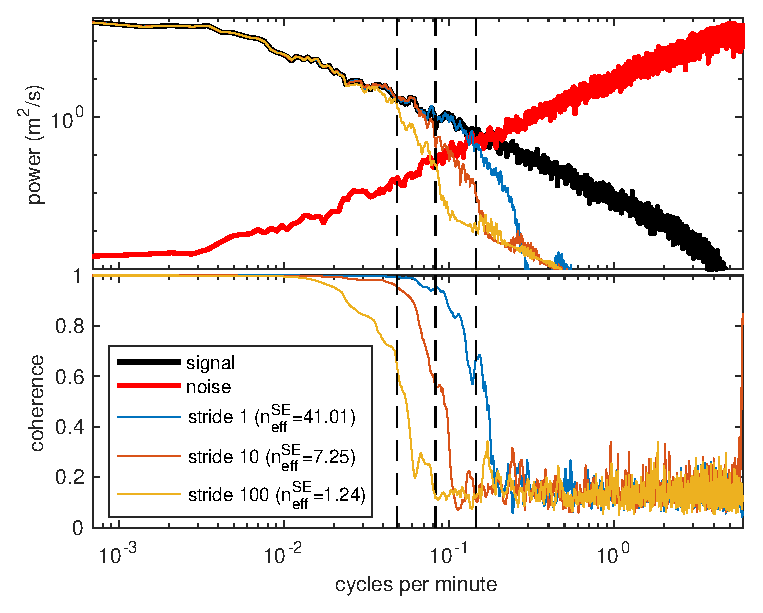
\includegraphics[width=19pc,angle=0]{figures/synthetic_process_and_spectrum_slope2degree3}}
  
  \caption{The upper panel shows the uncontaminated velocity spectrum of the signal (black) and velocity spectrum of the noise (red). The observed signal is the sum of the two. The blue, red, and orange lines show the spectrum of the tension spline best fit to the observations with all, 1/10th and 1/100th the data, respectively. The bottom panel shows the coherence between the smoothed signals and the true signal.}
  \label{synthetic_process_and_spectrum}
\end{figure}


%%%%%%%%%%%%%%%%%%%%%%
\subsection{Reduced spline coefficients} \label{reduced_coefficients}
%%%%%%%%%%%%%%%%%%%%%%

One practical consideration when working with large datasets is that the computational cost of creating the spline fit may be limited by the rate of solving for the spline coefficients. It is therefore beneficial to reduce knot points (and therefore total splines) when possible. A reasonable hypothesis is to suppose that when the effective sample size is large, as measured by equation \ref{dof_se}, that we may be able to avoid placing a knot point at every data point---essentially `skipping' data points.

To test this idea, we find the optimal fit over a range of different strides (which varies the effective sample size) and increase the number of knot points that are skipped until the mean square error starts to rise. We find that we can safely skip $\textrm{max}(1,\textrm{floor}(2n_{\textrm{eff}}/3))$ knot points without sacrificing any precision. In fact, as can be seen in table \ref{fit_results_gaussian}, in some cases the optimal mean square error improves with fewer knot points. The `full dof' column indicates a fit where one knot point is created for every observation point, whereas the `reduced dof' indicates a fit where the number of knot points is reduced.

This means that when handling large datasets, we can reduce the number of splines being used if the effective sample size is large, and we can simply `chunk' the data (split it into multiple independent pieces) if the effective sample size is small.

%%%%%%%%%%%%%%%%%%%%%%
\subsection{Interpolation condition} \label{interpolation_condition}
%%%%%%%%%%%%%%%%%%%%%%

To estimate the value of $\lambda_T$ from equation \ref{lambda}, we require an estimate of the mean-square value of a derivative of the process, $x_{\textrm{rms}}^{(T)}$ as well as an estimate of the effective sample size, $n_{\textrm{eff}}$. Assuming one can make an estimate of $x_{\textrm{rms}}^{(m)}$ from the signal (see appendix \ref{sec:variance_estimate}), we just need a method for estimating the effective sample size.

We argue that the effective sample size should vary based on the relative size of the measurement errors to the speed of motion. For example, if the position errors are only $1$ meter, but a particle typically travels $10$ meters between measurements, then it is hardly justifiable to increase the tension so that the smoothing spline misses the observation points by $1$ meter. There is not enough statistical evidence to suggest that the particle didn't go right through the observation point. On the other hand, if the position errors are $1$ meter, but particle typically travels $10$ centimeters between measurements, nearby measurements provide more information about the particle's true position during that time, so our estimate of the particle's true position is closer to a mean of the nearby observations.

This idea can be made more rigorous by noting that one would consider change in position, $\Delta x$, statistically significant if it exceeds the position errors, $\sigma_x$ by some factor.  Assuming the physical process has a characteristic velocity scale, $u_{\textrm{rms}}$, we use this concept to define $\Gamma$ as
\begin{equation}
\label{gamma_def}
\Gamma \equiv \frac{\sigma_x}{u_{\textrm{rms}}\Delta t}
\end{equation}
where $\sigma_x$ is the standard deviation of positioning noise and $\Delta t$ is the typical time between observations. This argument suggests that the effective sample size should be proportional to $\Gamma$, i.e.,
\begin{equation}
\label{gamma_equation}
n_{\textrm{eff}}^\Gamma = \max\left(1,C \cdot \Gamma^m\right)
\end{equation}
where $C$ and $m$ are unknown constants and we prevent the effective sample size from dropping below 1. Intuitively this means that as long as the particle didn't move too far between observations, nearby observations help to estimate the true position of the particle.

To test the relationship between $\Gamma$ and the effective sample size, we compute the optimal tension spline for a range of values of $\Gamma$ (created by sub-sampling the signal) for the three different slopes ($\omega^{-2}$, $\omega^{-3}$, $\omega^{-4}$). The value $n_{\textrm{eff}}^\textrm{SE}$ is computed from the optimal solution for 50 ensembles and shown in figure \ref{dofVsGamma}. The fits are remarkably good, but depend on the slope of process. Processes with shallower slopes (rougher trajectories) provide a smaller effective sample size for a given value of $\Gamma$. 

\begin{figure}
  \centerline{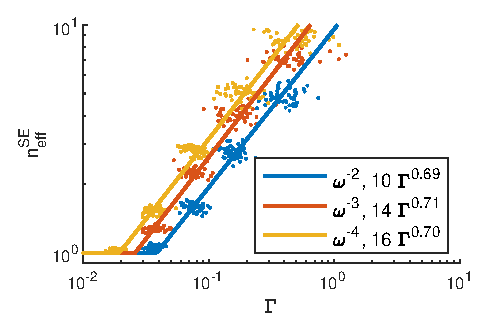
\includegraphics[width=19pc,angle=0]{figures/dofVsGamma}}
  
  \caption{Effective sample size from the standard error vs $\Gamma$}
  \label{dofVsGamma}
\end{figure}

Thus, using the interpolation condition $\Gamma$ to estimate the effective sample size, we set $n_{\textrm{eff}}^\Gamma = 14 \cdot \Gamma^{0.71}$, the empirically determined best fit for slope $\omega^{-3}$.  For all spline fits then, we use
\begin{equation}
\label{lambda_initial_guess}
\lambda^{\textrm{initial}}_T = \frac{n_{\textrm{eff}}^\Gamma-1}{n_{\textrm{eff}}^\Gamma} \frac{1}{ \left(x^{(T)}_{\textrm{rms}}\right)^2  T}
\end{equation}
as an initial estimate for the optimal smoothing parameter where both $x^{(T)}_{\textrm{rms}}$ and $u_\textrm{rms}$ are estimated using the method described in appendix \ref{sec:variance_estimate}.

The scaling law for $n_{\textrm{eff}}^\Gamma$ can be found analytically. Given a particle moving at some velocity $u_\textrm{rms}$, observed at regular intervals of $\Delta t$ with position error $\sigma$, what is the expected number of samples $\left\langle n \right\rangle$ for a statistically significant change in position? Specifically, let the position observations be given by $x_i$ where
\begin{equation}
x_i = u_\textrm{rms} i \Delta t + \epsilon_i \textrm{ where } \epsilon_i = \mathcal{N}(0,\sigma).
\end{equation}
If the effective sample size is $\left\langle n \right\rangle$, then the particles changes position by $\left\langle n \right\rangle u_\textrm{rms} \Delta t$ between samples. Applying the two-sample z-test two positions will be considered different for $z>z_\textrm{min}$ where
\begin{equation}
z= \frac{\left\langle n \right\rangle u_\textrm{rms} \Delta t}{\sqrt{\frac{\sigma^2}{\left\langle n \right\rangle} + \frac{\sigma^2}{\left\langle n \right\rangle} }}
\end{equation}
or,
\begin{equation}
\label{gamma_analytical}
\left\langle n \right\rangle = \left( \frac{z \sigma \sqrt{2}}{u_\textrm{rms} \Delta t} \right)^{\frac{2}{3}}.
\end{equation}
The power law in equation \ref{gamma_analytical} matches the empirically derived power laws shown in figure \ref{dofVsGamma} and suggests that $m$ in equation \ref{gamma_equation} should be $m=2/3$. This also suggests that the coefficient $C$ in equation \ref{gamma_equation} can be related $z$, a measure of statistical significance.

%  To estimate the tension parameter $\lambda_2$ from equation \ref{lambda} we therefore need an estimate of both $u_{\textrm{rms}}$ and $a_{\textrm{rms}}$. Computing this directly from the observed signal in the time domain is problematic because, given frequent enough sampling, the noise will dominate the estimate. Instead we estimate these values in the frequency domain summing the power in the frequency bins that more than 10 times the expected value of the noise. Because each frequency bin in a periodigram follows a $\chi^2$ distribution for two degrees of freedom, this only adds observed power that is likely to be true signal.



%%%%%%%%%%%%%%%%%%%%%%
\subsection{Optimal fits} \label{optimal_fits}
%%%%%%%%%%%%%%%%%%%%%%

\begin{table}[ht]
\caption{Mean square error and effective sample size for a range of strides. The first three columns show the baseline optimal, best-case scenario found using the uncontaminated signal with 1 knot point for each point (1 dof). The next three columns show the average increase in mean-square error. The `reduced dof' column shows the optimal value after reducing the number of knot points using the effective degrees of freedom in section \ref{reduced_coefficients}. The `blind initial' column uses equation \ref{lambda_initial_guess} to set $\lambda_T$, while the `expected mse' column optimizes using equation \ref{MSE} }
\label{fit_results_gaussian}
\centering
\begin{tabular}{r r p{1cm} | p{1cm}p{1cm}p{1cm}p{1cm}} stride & $n_\textrm{eff}$ & optimal mse & reduced dof & blind initial & expected mse \\ \hline \hline 
$\omega^{-2}$ &&&&&  \\ \hline 
1 & 8.6 & 11.5 m$^2$ &  0.1\%  &  56.4\%  &  7.4\%  \\ 
2 & 4.9 & 20.4 m$^2$ &  0.0\%  &  36.3\%  &  2.8\%  \\ 
4 & 2.9 & 34.2 m$^2$ &  0.1\%  &  20.0\%  &  1.7\%  \\ 
8 & 1.7 & 55.9 m$^2$ &  0.0\%  &  5.6\%  &  1.0\%  \\ 
16 & 1.2 & 81.8 m$^2$ &  0.0\%  &  3.6\%  &  0.5\%  \\ 
$\omega^{-3}$ &&&&&  \\ \hline 
1 & 12.5 & 7.64 m$^2$ &  -0.1\%  &  38.6\%  &  6.4\%  \\ 
2 & 7.1 & 13.4 m$^2$ &  -0.1\%  &  20.4\%  &  3.5\%  \\ 
4 & 4.1 & 23.5 m$^2$ &  -0.0\%  &  9.8\%  &  2.2\%  \\ 
8 & 2.3 & 41.8 m$^2$ &  0.0\%  &  1.7\%  &  1.2\%  \\ 
16 & 1.4 & 67.9 m$^2$ &  0.0\%  &  9.6\%  &  0.6\%  \\ 
$\omega^{-4}$ &&&&&  \\ \hline 
1 & 15.6 & 5.69 m$^2$ &  -0.1\%  &  33.8\%  &  7.9\%  \\ 
2 & 9.0 & 10.5 m$^2$ &  -0.1\%  &  18.6\%  &  5.1\%  \\ 
4 & 5.0 & 18.6 m$^2$ &  -0.0\%  &  8.6\%  &  2.4\%  \\ 
8 & 2.8 & 33.2 m$^2$ &  0.0\%  &  3.2\%  &  1.5\%  \\ 
16 & 1.6 & 57.6 m$^2$ &  0.0\%  &  15.4\%  &  0.8\%  \\ 
\end{tabular} 

\end{table}


Table \ref{fit_results_gaussian} summarizes the key results of this section by applying a tension spline with with $S=3$ to the 200 ensembles of the noise and signal with three different slope ($\omega^{-2}$, $\omega^{-3}$, $\omega^{-4}$) and five different strides. The first column shows the average mean square error and effective sample size when the tension spline is applied using the true values to minimize the mean square error---this is the lower bound. The second column shows average increase in mean-square error when reducing the number of spline coefficient as document in section \ref{reduced_coefficients}. There is almost no change mean-square error. The third column uses equation \ref{lambda_initial_guess} from section \ref{interpolation_condition} to provide a (blind) initial guess of the tension parameter. Here the results are mixed---a typical increase in mean-square error is about 30-50\% when the effective sample size is large. While this might seem large, this is a small fraction of the total variance of the noise, e.g., an optimal mean square error of $6$ m$^2$ increase to $8$ m$^2$ when the total variance is $100$ m$^2$. When the data sets are small (and computation time isn't a limiting factor), nearly optimal fits can be found using equation \ref{MSE}, as shown in the last column of the table.

For point of comparison, table \ref{fit_results_gaussian_other_methods} shows shows the relative performance of other minimization methods compared to the expected mean-square error method, equation \ref{MSE}.  The relative performance of cross-validation (cv), generalized cross-validation (gcv), and the log-likelihood method (equation \ref{gaussian-max-likelihood}) are all remarkably good. Cross-validation and generalized cross-validation perform similar to each other, and similar to the expected mean-square error for larger effective sample sizes. The cross-validation methods start to fall-apart as the effective sample size decreases towards 1 (which is clear from their definition must happen). The log-likelihood method requires knowing $\sigma$ and estimating $x_\textrm{rms}^{(T)}$ (see appendix \ref{sec:variance_estimate}), which makes the method somewhat less practical unless both happen to be known.

\begin{table}[ht]
\caption{Mean square error and effective sample size for a range of strides.  The first three columns show the baseline values using the expected MSE (equation \ref{MSE}) to minimize. The next four columns show the average increase in mean-square error. The `ranged mse' column uses the ranged expected mse described in section \ref{sec:robust_minimization}. The `cv' column uses cross-validation (equation 3.5 in \cite{green1994-book}).  The `cv' column uses generalized cross-validation (equation 3.13 in \cite{green1994-book}) and the `log-likelihood' column uses equation \ref{gaussian-max-likelihood}.}
\label{fit_results_gaussian_other_methods}
\centering
\begin{tabular}{r p{1cm} | p{1cm}p{1cm}p{1cm}p{1cm}} $n_\textrm{eff}$ (stride) & expected mse & ranged & cv & gcv & log-likelihood \\ \hline \hline 
$\omega^{-2}$ &&&&&  \\ \hline 
8.6 (1) & 12.4 m$^2$ &  3.0\% &  0.2\% &  0.5\% & 5.8\% \\ 
5.0 (2) & 21.0 m$^2$ &  2.1\% &  1.1\% &  0.6\% & 15.9\% \\ 
2.9 (4) & 34.8 m$^2$ &  1.1\% &  0.7\% &  0.4\% & 16.6\% \\ 
1.7 (8) & 56.4 m$^2$ &  0.4\% &  1.5\% &  0.9\% & 6.4\% \\ 
1.2 (16) & 82.2 m$^2$ &  0.1\% &  17.5\% &  19.4\% & 1.7\% \\ 
$\omega^{-3}$ &&&&&  \\ \hline 
12.6 (1) & 8.11 m$^2$ &  1.8\% &  -0.0\% &  -0.3\% & 7.6\% \\ 
7.1 (2) & 13.9 m$^2$ &  3.3\% &  0.6\% &  0.2\% & 7.5\% \\ 
4.0 (4) & 24.0 m$^2$ &  1.1\% &  0.7\% &  0.2\% & 8.5\% \\ 
2.3 (8) & 42.3 m$^2$ &  0.7\% &  1.2\% &  0.6\% & 0.6\% \\ 
1.4 (16) & 68.4 m$^2$ &  0.3\% &  9.0\% &  6.8\% & 2.9\% \\ 
$\omega^{-4}$ &&&&&  \\ \hline 
15.7 (1) & 6.15 m$^2$ &  5.5\% &  1.0\% &  0.3\% & 19.2\% \\ 
9.0 (2) & 11.0 m$^2$ &  2.8\% &  1.0\% &  1.2\% & 9.0\% \\ 
5.1 (4) & 19.1 m$^2$ &  1.0\% &  0.2\% &  0.0\% & 7.4\% \\ 
2.8 (8) & 33.7 m$^2$ &  1.0\% &  1.2\% &  0.6\% & 5.4\% \\ 
1.6 (16) & 58.1 m$^2$ &  0.3\% &  4.8\% &  2.4\% & 10.2\% \\ 
\end{tabular} 

\end{table}

%%%%%%%%%%%%%%%%%%%%%%
\section{Bivariate tension splines and stationarity}
\label{sec:bivariate}
%%%%%%%%%%%%%%%%%%%%%%

The term `bivariate' in the context of splines is often used to denote splines defined on two independent variables---however, in this context we define bivariate to mean two dependent variables (e.g., $x$ and $y$) and one independent variable (e.g., $t$).

The trivial approach to working with such bivariate data is to treat each direction independently---i.e., minimize $\lambda^x_T$ and $\lambda^y_T$ independently of each other. However, the more physically interesting case is when the underlying process is suspected of being isotropic. In the context of the maximum likelihood formulation of tension spline, equation \ref{smoothing-spline-pdf}, this means that we expected $x^{(T)}_{\textrm{rms}}$ (the rms value of the tensioned variable) to be the same in all directions (invariant under rotation). Note, however, that this does \emph{not} mean that $\lambda_x$ should necessarily equal $\lambda_y$. To be explicit, if 
\begin{align}
\label{lambda_x}
\lambda^x_T =& \frac{n^x_{\textrm{eff}}-1}{n^x_{\textrm{eff}}} \frac{1}{ \left(x^{(T)}_{\textrm{rms}}\right)^2 (t_N-t_1)} \textrm{ and}\\
\lambda^y_T =& \frac{n^y_{\textrm{eff}}-1}{n^y_{\textrm{eff}}} \frac{1}{ \left(y^{(T)}_{\textrm{rms}}\right)^2 (t_N-t_1)}
\end{align}
then even if $x^{(T)}_{\textrm{rms}} = y^{(T)}_{\textrm{rms}}$, the effective sample sizes $n^x_{\textrm{eff}}$ and $n^y_{\textrm{eff}}$ will not necessarily be equal if there is any mean velocity because, as shown in section \ref{interpolation_condition}, the effective sample size depends on velocity.

To assume isotropy in $\lambda_T$ and use a bivariate tension spline, the mean velocity from the underlying process must be removed. What qualifies as mean and fluctuation rarely has a clear answer, but a reasonable option to consider is letting a polynomial of degree $T$ define the mean. This has the added benefit of removing a constant non-zero tension value, which as shown in section \ref{sec:maximum_likelihood}, changes the problem formulation. 

It's worth noting that it is not actually isotropy that requires removing the mean velocity, but in fact stationarity. The effective sample size is shown to be dependent on rms velocity, so if the velocity varies in time, then the optimal effective sample size will need to vary as well. This means that not only do tension splines require stationarity in the tensioned variable $x^{(T)}$ as shown in section \ref{sec:maximum_likelihood}, but they also require stationarity in the velocity $x^{(1)}$ to be effective. This last requirement can be solved be either removing the mean (as we have suggested), or segmenting observations into pseudo-stationary chunks.

%%%%%%%%%%%%%%%%%%%%%%
\subsection{Assessing errors}
\label{sec:errors_wit_mean}
%%%%%%%%%%%%%%%%%%%%%%

Removing the mean or some other low-passed version of the data means that the total smoothing matrix will be some combination of the low-passed and high-passed smoothing matrices. Once this matrix is computed, it can be used to compute the standard errors.

We first create a low pass filter to capture the \emph{mean} component of the flow using a simple polynomial fit,
\begin{equation}
\bar{\mathbf{x}} = \bar{\mathbf{S}} \mathbf{x}
\end{equation}
and then define the residual as our stationary part,
\begin{equation}
\mathbf{x}^\prime \equiv \mathbf{x} - \bar{\mathbf{x}}.
\end{equation}
We now compute the tension spline as usual on the residual,
\begin{equation}
\mathbf{x}^\prime_\lambda = \mathbf{S}_\lambda \mathbf{x}^\prime
\end{equation}
So the total, smoothed path is
\begin{align}
\hat{\mathbf{x}} =& \bar{\mathbf{x}} + \mathbf{x}^\prime_\lambda \\
=& \bar{\mathbf{S}} \mathbf{x} + \mathbf{S}_\lambda \left( \mathbf{x} - \bar{\mathbf{S}} \mathbf{x} \right) \\
=& \left(\bar{\mathbf{S}} + \mathbf{S}_\lambda - \mathbf{S}_\lambda \bar{\mathbf{S}}\right)\mathbf{x} \\
\equiv& \mathbf{S}_T \mathbf{x}
\end{align}
From this we can easily compute the covariance matrix and the standard error.

%%%%%%%%%%%%%%%%%%%%%%
\section{GPS data set}
\label{sec:drifter_data_set}
%%%%%%%%%%%%%%%%%%%%%%

The GPS positions used in this manuscript were collected from oceanic surface \emph{drifters}, floating buoys with drogues tethered 15-30 meters below the ocean surface, depending on the particular experiment being conducted. In the past, these drifters have used Argos positioning system which has significantly poorer temporal coverage and position accuracy \cite{elipot2016-jgr}, but recently more surface drifters have employed GPS receivers and transmitted their data back through Argos or Iridium satellites.

The primary dataset considered here will be nine surface drifters that were deployed in the Sargasso Sea in the summer of 2011. These particular drifters were part of the LatMix experiment \cite{shcherbina2015-bams} and recorded data at approximately 30 minute intervals over the course of a week before being retrieved.

The GPS receiver sits on the surface buoy and collects position data, but because of atmospheric conditions or ocean waves, the receivers are sometimes unable to obtain a position, or when they do, it is highly inaccurate. Thus, despite nominal accuracies of a few meters, it is often the case that some positions are off by more than 1000 meters, as can be seen in figure \ref{gpsfit}. Taking $\sigma=10$ meters and applying a tension spline fit using the methodology in section \ref{sec:smoothing_spline} produces an obviously horrible fit, with clear overshoots to bad data points.

In the following two sections we examine the expected errors from GPS position data and test the effectiveness of tension splines with non-Gaussian errors.

%%%%%%%%%%%%%%%%%%%%%%
%
\subsection{GPS error distribution}
\label{gps_position_errors}
%
%%%%%%%%%%%%%%%%%%%%%%

\begin{figure}
  \centerline{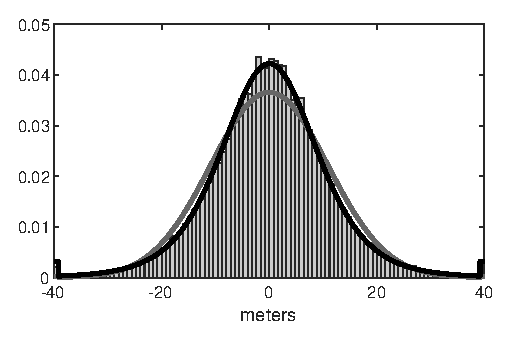
\includegraphics[width=19pc,angle=0]{figures/gps_error_distribution}}
  \centerline{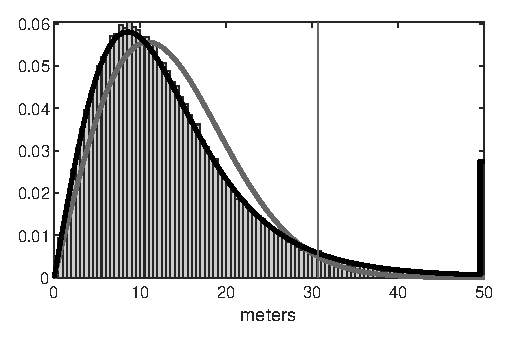
\includegraphics[width=19pc,angle=0]{figures/gps_distance_error_distribution}} 
  \caption{The top panel shows the position error distribution of the motionless GPS. The black line is the best fit t-distribution and the gray line is the best fit Gaussian distribution. The bottom panel shows the distance error distribution with the corresponding expected distributions from the Gaussian and t-distribution. The vertical line in the bottom panel shows the 95\% error of the t-distribution at about 30 meters.}
  \label{motionless_error}
\end{figure}

We characterize the the GPS errors by considering data from a motionless GPS receiver allowed to run for 12 hours. The specific GPS receiver used for this test was not the same as the one used for the drifters (because it was no longer available) but should produce errors similar enough for this analysis.

The position recorded by the motionless GPS are assumed to have isotropic errors with mean zero, which means that the positions themselves are the errors. The probability distribution function (PDF) of the combined $x$ and $y$ position errors are shown in figure \ref{motionless_error}.

The error distribution is first fit to a zero-mean Gaussian PDF,
\begin{equation}
\tag{\ref{gaussian_pdf} revisited}
p_g(\epsilon|\sigma_g) = \frac{e^{-\frac{1}{2}\frac{\epsilon^2}{\sigma_g^2}} }{\sigma_g \sqrt{ 2 \pi}}.
\end{equation}
The maximum likelihood fit is found by simply computing the standard deviation of the sample, which is found to be $\sigma_g \approx 10$ meters and shown as the gray line in figure \ref{motionless_error}. However, it is clear the error distribution shows much longer tails than the Gaussian PDF.

The Student t-distribution is a generalization of the Gaussian that produces longer tails and is defined as 
\begin{equation}
\label{student_pdf}
p_t\left(\epsilon |\nu,\sigma_t^2\right) = \frac{\Gamma\left( \frac{\nu + 1}{2} \right)}{\sigma_t \sqrt{\nu \pi} \Gamma\left(\frac{\nu}{2}\right)} \left( 1 + \frac{\epsilon^2}{\sigma_t^2 \nu} \right)^{-\frac{\nu+1}{2}}
\end{equation}
where the $\sigma_t$ parameter scales the distribution width and the $\nu$ parameter sets the number of degrees of freedom. The variance is $\textrm{var}(X)=\sigma_t^2 \frac{\nu}{\nu-2}$ and only exists for $\nu > 2$. The t-distribution is equivalent to the Gaussian distribution when $\nu \rightarrow \infty$. We find the best fit t-distribution to the data by minimizing the Anderson-Darling test. The best fit with parameters $\sigma_t \approx 8.5$ meters and $\nu \approx 4.5$ is shown as the black line in figure \ref{motionless_error}. Different choices in GPS receivers and using the Kolmogorov-Smirnoff test results in very similar parameters, i.e., $\sigma_t\approx8-10$ meters and $\nu\approx4-6$.

The \emph{position} error distributions also imply a combined \emph{distance} error distribution by computing $\epsilon_d = \sqrt{\epsilon_x^2 + \epsilon_y^2}$ and is shown in the lower panel of figure \ref{motionless_error}. For two independent Gaussian distributions this results in a Rayleigh distribution,
\begin{equation}
\label{rayleigh_pdf}
p_r(\epsilon_d|\sigma_g) = \frac{\epsilon_d}{\sigma_g^2 } e^{-\frac{1}{2}\frac{\epsilon_d^2}{\sigma_g^2}}.
\end{equation}
The distance distribution for two t-distributions is computed numerically and is shown in the bottom panel of figure \ref{motionless_error} on top of the actual distance errors. Approximately 95\% of distance errors are within $30$ meters, shown as the vertical gray line in figure \ref{motionless_error}.

\begin{figure}
  \centerline{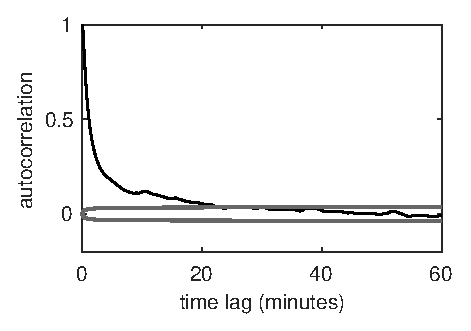
\includegraphics[width=19pc,angle=0]{figures/gps_autocorrelation}}
  \caption{The autocorrelation function of the GPS positioning error with 99\% confidence intervals shown in gray. The correlation at drifter sampling period of 30 minutes is indistinguishable from zero.}
  \label{gps_autocorrelation}
\end{figure}

Figure \ref{gps_autocorrelation} shows the autocorrelation function of the GPS position errors. We find rough empirical fit to be $\rho(\tau)=\exp\left(\max(-\tau/t_0,-\tau/t_1-1.35)\right)$ where $t_0=100$ seconds and $t_1=760$ seconds, which reflects an initially rapid fall off in correlation, followed by a slower decline. The smallest sampling interval of the GPS drifters in question is 30 minutes and therefore it is safe to assume the errors are uncorrelated for our purposes.

The tension spline algorithms described in section \ref{sec:smoothing_spline} are modified to use the Student t-distribution as described in section \ref{sec:irls}. Table \ref{fit_results_tdistribution} shows that the conclusions reached for Gaussian data in section \ref{sec:smoothing_spline} still apply to the t-distribution data used here.

\begin{table}[ht]
\caption{Same as table \ref{fit_results_gaussian}, but with noise following Student-t distribution.}
\label{fit_results_tdistribution}
\centering
\begin{tabular}{r r p{1cm} | p{1cm}p{1cm}p{1cm}p{1cm}} stride & $n_\textrm{eff}$ & optimal mse & reduced dof & blind initial & expected mse \\ \hline \hline 
$\omega^{-2}$ &&&&&  \\ \hline 
1 & 8.2 & 11.8 m$^2$ &  0.3\%  &  66.7\%  &  7.7\%  \\ 
2 & 4.7 & 20.9 m$^2$ &  0.3\%  &  47.3\%  &  6.6\%  \\ 
4 & 2.8 & 38.0 m$^2$ &  0.1\%  &  24.2\%  &  4.4\%  \\ 
8 & 1.6 & 66.3 m$^2$ &  0.0\%  &  8.2\%  &  9.3\%  \\ 
16 & 1.2 & 101. m$^2$ &  0.0\%  &  8.1\%  &  3.7\%  \\ 
$\omega^{-3}$ &&&&&  \\ \hline 
1 & 12.1 & 7.51 m$^2$ &  -0.1\%  &  36.2\%  &  8.8\%  \\ 
2 & 6.8 & 13.4 m$^2$ &  -0.1\%  &  22.8\%  &  7.0\%  \\ 
4 & 3.9 & 26.0 m$^2$ &  -0.0\%  &  11.5\%  &  3.8\%  \\ 
8 & 2.2 & 47.5 m$^2$ &  0.0\%  &  2.2\%  &  3.2\%  \\ 
16 & 1.3 & 82.5 m$^2$ &  0.0\%  &  12.6\%  &  8.5\%  \\ 
$\omega^{-4}$ &&&&&  \\ \hline 
1 & 14.9 & 6.01 m$^2$ &  -0.2\%  &  35.3\%  &  9.0\%  \\ 
2 & 8.6 & 10.5 m$^2$ &  -0.2\%  &  24.8\%  &  7.0\%  \\ 
4 & 4.8 & 19.1 m$^2$ &  -0.1\%  &  7.8\%  &  4.6\%  \\ 
8 & 2.7 & 36.4 m$^2$ &  0.0\%  &  3.2\%  &  2.7\%  \\ 
16 & 1.6 & 69.1 m$^2$ &  0.0\%  &  18.9\%  &  11.5\%  \\ 
\end{tabular} 

\end{table}



%%%%%%%%%%%%%%%%%%%%%%
\section{Removing Outliers}
\label{sec:outliers}
%%%%%%%%%%%%%%%%%%%%%%

\begin{figure*}[t]
  \centering
    \begin{minipage}{0.35\textwidth}
        \centering
        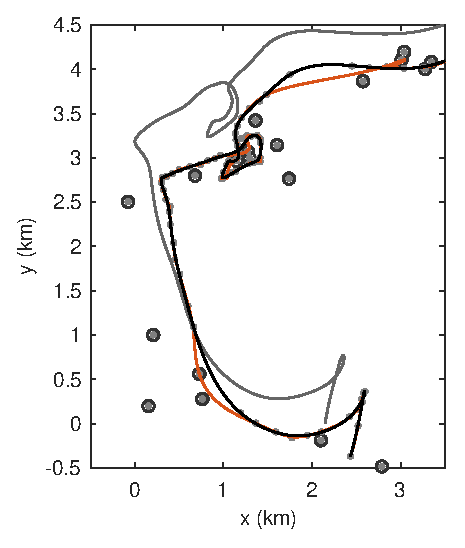
\includegraphics[width=1.0\textwidth]{figures/gpsfit_xy} % first figure itself
        % \caption{first figure}
    \end{minipage}\hfill
    \begin{minipage}{0.65\textwidth}
        \centering
        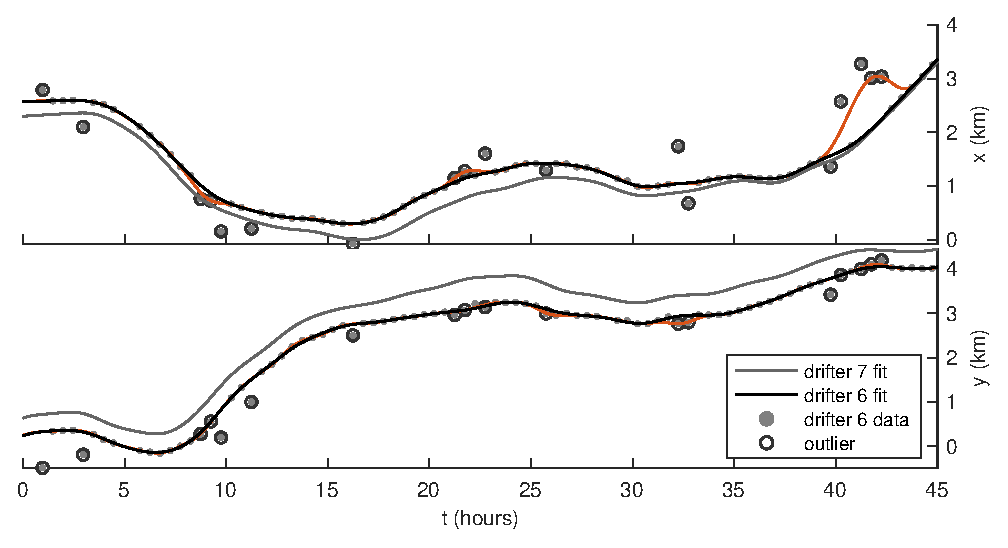
\includegraphics[width=1.0\textwidth]{figures/gpsfit_xtyt} % second figure itself
        % \caption{second figure}
    \end{minipage}
  
%   \caption{GPS position data for a 25 hour window from one of the drifters. The light grey line is the is optimal tension spline fit assuming Gaussian errors, as described in section \ref{sec:smoothing_spline}. The highlighted data points are those identified as outliers using the methodology in section \ref{sec:outliers}. The black line is the optimal tension spline fit assuming t-distribution errors after removing outliers following section \ref{sec:drifter_data_set}.}
  \label{gpsfit}
\end{figure*}

The goal here is to remove the outliers---points that do not appear to be of the known error distribution for the GPS receiver shown in section \ref{gps_position_errors}. These points are obviously bad as can be seen in figure \ref{gpsfit} where individual data points jump hundreds of meters and even several kilometers away from its neighbors. Errors of this size are inconsistent with the noise analysis of the preceding section, so the goal here is to identify points associated with this uncharacterized noise. What makes outliers `obvious' to the eye is that they appear as unexpectedly large motions, inconsistent with most of the other motion for that path. In this sense, the tension spline formulation is a good one as it assumes the motion at some order (e.g., acceleration) is Gaussian, as shown in section \ref{sec:maximum_likelihood}. Interestingly, in the nine drifters we are analyzing here, one drifter shows no obvious outliers, suggesting the issue may be related to how the antenna is configured. This particular drifter serves as a useful point of comparison.

The basic problem formulation is as follows: we define a new `robust distribution', $p_{\textrm{robust}}$, that includes the known noise distribution, $p_{\textrm{noise}}$, plus an unknown (or assumed) form of an outlier distribution, $p_{\textrm{outlier}}$,
\begin{equation}
\label{robust_pdf}
    p_{\textrm{robust}}(\epsilon) = (1-\alpha) \cdot p_{\textrm{noise}}(\epsilon) + \alpha \cdot  p_{\textrm{outlier}}(\epsilon).
\end{equation}
For this section we did not consider a normal distribution for $p_{\textrm{noise}}$, but considered only a Student's t-distribution with parameters found from the GPS errors in section \ref{gps_position_errors}. The distribution of $ p_{\textrm{outlier}}$ was also set to be a Student's t-distribution, but with $n=3$ and $\sigma=40\sigma_\textrm{gps}$ which roughly matches the total variance of the observed outliers. In our tests we varied $\alpha$ from 0 up to $0.25$, approximately the range of observed outliers from the drifter data sets.

Throughout our attempts to smooth the noisy GPS data we tried many different approaches to modifying tension splines for robustness to outliers, but ultimately, found that enormous gains in accuracy are made by simply discarding outliers while minimizing the expected mean square error, equation \ref{MSE}. The results of this approach are shown in section \ref{sec:robust_minimization}, but we also document our methodology to reliably estimate the outlier distribution in section XX.

%%%%%%%%%%%%%%%%%%%%%%
\subsection{Robust minimization}
\label{sec:robust_minimization}
%%%%%%%%%%%%%%%%%%%%%%

The whole problem with outliers is that we don't know their distribution, so minimizing the expected mean square error using equation \ref{MSE} with the expected variance from the robust distribution defined in equation \ref{robust_pdf} cannot possibly work. Outliers add extra variance, and will therefore cause the spline to be under tensioned. The key idea in our method is to simply exclude the outliers from the calculation of equation \ref{MSE}, where outliers are defined as points unlikely to arise with the known noise distribution. The robust expected mean square error thus replaces $\sigma^2$ with,
\begin{equation}
    \sigma^2 = \int_{\textrm{cdf}^{-1}(\alpha/2)}^{\textrm{cdf}^{-1}(1-\alpha/2)} z^2 p_{\textrm{noise}}(z) \, dz
\end{equation}
and discards all rows (and columns) of $\mathbf{S}_\lambda$ where $\left(\mathbf{S}_\lambda - I\right)\mathbf{x}<\textrm{cdf}^{-1}(\alpha/2)$ or $\left(\mathbf{S}_\lambda - I\right)\mathbf{x}>\textrm{cdf}^{-1}(1-\alpha/2)$.

Table \ref{fit_results_gaussian_other_methods} shows the results of applying this method to data without outliers. The results show a modest increase in mean square error in the worst case scenario.

To test this approach we generate data as before, but now also let a certain percentage of outliers ($\alpha$) be generated with an outlier distribution. Results are shown here.

%%%%%%%%%%%%%%%%%%%%%%
\subsection{Full tension solution and outlier distribution}
\label{sec:full_tension}
%%%%%%%%%%%%%%%%%%%%%%

The \emph{full tension} solution is defined as the maximum allowable value of lambda given the known noise distribution. That is, the spline fit is pulled away from the observations so that that the distribution of observed errors ($x_i-x(t_i)$) matches the expected distribution $p_{\textrm{noise}}(\epsilon)$. In cases where the effective sample size $n_\textrm{eff}$ is large, the full tension solution will approximately match the optimal (minimal mean square error) solution. In cases where the effective sample size is closer to one, the full tension solution is more akin to a low-pass solution (because increasing $\lambda$ is equivalent to decreasing $x^{(T)}_\textrm{rms}$.

In the simplest case where there are no outliers the full tension solution can be found by requiring that the sample variance match the variance of $p_{\textrm{noise}}(\epsilon)$. When outliers are present, a more robust method of estimation is required. After some experimentation, we found that the most reliable method of achieving full tension is to minimize the Anderson-Darling test of $p_{\textrm{noise}}(\epsilon)$ on the interquartile of observed errors. In fact, we found that this method can be used to estimate the outlier distribution and further refine both the full tension solution and range over which the expected mean square error is computed.

The outlier distribution is estimated in the following fashion. We first assume that the outlier distribution follows a Student's t-distribution with $\nu=3$ and that $\alpha<0.5$. If the spline is in full tension, then the observed total variance can be used to find $\sigma_o$ for the outlier distribution. From equation \ref{robust_pdf} it follows that,
\begin{equation}
    \textrm{var}_\textrm{total} = (1-\alpha) \textrm{var}_\textrm{noise} + \alpha 3 \sigma_o^2
\end{equation}
which, given some $\alpha$, can be solved for $\sigma_o$. Our method considers 100 different values of alpha logarithmicaly spaced from $0.01$ to $0.5$ and chooses the value which minimizes the Anderson-Darling test.

With an estimate for $p_{\textrm{robust}}(\epsilon)$, the the full tension solution can be refined by now minimizing the Anderson-Darling test of $p_{\textrm{robust}}(\epsilon)$ on the interquartile of observed errors. This iterative process converges quite quickly on both a good estimate for the outlier distribution and the full tension solution.


%%%%%%%%%%%%%%%%%%%%%%
\subsection{Extension to bivariate data}
\label{sec:robust_bivariate}
%%%%%%%%%%%%%%%%%%%%%%

The strategies in this section are relatively easily extended to bivariate data. All error distribution are assumed isotropic, and thus the outlier distribution can be estimated by including the errors from both independent directions.

The ranged expected mean-square error calculation uses the \emph{distance} of the error for its cutoff in order to remain invariant under rotations. The pdf crossover point is found using the two-dimensional distance distribution empirically computed from the one-dimension noise and outlier distributions.

%%%%%%%%%%%%%%%%%%%%%%
\section{Conclusions}
%%%%%%%%%%%%%%%%%%%%%%

- we avoided autocorrelation, although it's very addressable.
- method has strong limitations: stationarity assumptions in particular.
- notice that ultimately we avoid using any interpolation from the interpolating spline, in the sense that we're not using information between the data points. That said, we're still using the 

%%%%%%%%%%%%%%%%%%%%%%
%
\appendices
%
%%%%%%%%%%%%%%%%%%%%%%

%%%%%%%%%%%%%%%%%%%%%%
\section{Numerical implementation}
\label{sec:numerical_implementation}
%%%%%%%%%%%%%%%%%%%%%%

The B-splines are generated using the algorithm described in \cite{deboor1978-book} with knot points determined by equations \ref{even-knots} and \ref{odd-knots}. The matrix $\mathbf{X}$ with components $X\indices{^i_m}$ denotes the $m$-th B-spline at time $t_i$. The first, second and third derivatives of the B-splines are denotes by $V\indices{^i_m}$, $A\indices{^i_m}$, $J\indices{^i_m}$, denoting velocity, acceleration, and jerk, respectively. In this notation the column vector $\xi^m$ represents the coefficients of the splines such that positions at time $t_i$ are given by $\hat{x}^i$ where $\hat{x}^i =  X\indices{^i_m} \xi^m$.

The discretized the penalty function is
\begin{equation}
\begin{split}
\phi = \left[ x^k - X\indices{^k_j} \xi^j \right]^{\textrm{T}} \left(\Sigma^{-1}\right)\indices{^k_i} \left[ x^i - X\indices{^i_l} \xi^l \right] \\
+ \lambda_1 \left[V\indices{^q_j} \xi^j \right]^{\textrm{T}} \left[ V\indices{^q_l} \xi^l \right]
\end{split}
\end{equation}
or
\begin{equation}
\phi = \left[ \mathbf{x} - \mathbf{X} \mathbf{\xi} \right]^{\textrm{T}} \Sigma^{-1} \left[ \mathbf{x} - \mathbf{X} \mathbf{\xi}\right]
+ \lambda_1 \left[\mathbf{V}\mathbf{\xi} - \mu \right]^{\textrm{T}} \left[ \mathbf{V}\mathbf{\xi} - \mu \right]
\end{equation}
where $\Sigma$ denotes the covariance matrix describing the measurement errors.

To find the coefficients that minimize this function, we take the derivative with respect to $\xi^m$, set it equal to zero, and solve for $\xi^m$,
\begin{equation}
\begin{split}
\xi^m = \left[ X\indices{_k_j} \left(\Sigma^{-1}\right)\indices{^k_i}  X\indices{^i_m} + \lambda_1 {A}\indices{^q_j}{A}\indices{^q_m} \right]^{-1} \\
\cdot x_k \left(\Sigma^{-1}\right)\indices{^k_i}   X\indices{^i_j}.
\end{split}
\label{solution}
\end{equation}
or
\begin{equation}
\label{solution2}
\mathbf{\xi} = \left[ \mathbf{X}^{\textrm{T}} \Sigma^{-1} \mathbf{X} + \lambda_1 \mathbf{V}^{\textrm{T}} \mathbf{V} \right]^{-1} \mathbf{X}^{\textrm{T}} \Sigma^{-1} \mathbf{x}
\end{equation}

This means that,
\begin{equation}
\mathbf{\hat{x}} = \mathbf{S_\lambda} \mathbf{x}
\end{equation}
where we've defined the smoothing matrix
\begin{equation}
\label{smoothing-operator}
\mathbf{S_\lambda} \equiv \mathbf{X} \left[ \mathbf{X}^{\textrm{T}} \Sigma^{-1} \mathbf{X} + \lambda_1 \mathbf{V}^{\textrm{T}} \mathbf{V} \right]^{-1} \mathbf{X}^{\textrm{T}} \Sigma^{-1}.
\end{equation}
which takes observations $\mathbf{x}$ to their smoothed values $\mathbf{\hat{x}}$.

The first matrix on the right hand side of equation \ref{solution} is $N\times N$ and fully invertible because the knots point were chosen such that each spline has at least one data point in its nonzero region. This is a nice feature because it means the solution will be well-behaved even if there is no tension.

The tension spline condition given in \ref{gaussian-max-likelihood} can be augmented to include a nonzero mean tension, $\mu_u$,
\begin{equation}
\phi =  \frac{d}{d-1} \frac{1}{N} \sum^N _{i=1}\left( \frac{x_i - x(t_i)}{\sigma_i} \right)^2 + \frac{1}{Q} \sum^{Q}_{q=1}  \left(  \frac{u(t_q)-\mu_u}{\sigma_u} \right)^2.
\end{equation}
When discretized, this penalty function becomes
\begin{equation}
\phi = \left[ \mathbf{x} - \mathbf{X} \mathbf{\xi} \right]^{\textrm{T}} \Sigma^{-1} \left[ \mathbf{x} - \mathbf{X} \mathbf{\xi}\right]
+ \lambda_1 \left[\mathbf{V}\mathbf{\xi} - \mu \right]^{\textrm{T}} \left[ \mathbf{V}\mathbf{\xi} - \mu \right]
\end{equation}
which has solution
\begin{equation}
\mathbf{\xi} = \left[ \mathbf{X}^{\textrm{T}} \Sigma^{-1} \mathbf{X} + \lambda_1 \mathbf{V}^{\textrm{T}} \mathbf{V} \right]^{-1}   \left[ \mathbf{X}^{\textrm{T}} \Sigma^{-1} \mathbf{x} +  \mu \lambda_1 \mathbf{V}^{\textrm{T}} \mathbf{\iota} \right]
\end{equation}
where $\mathbf{\iota}$ is a vector of $1$s. The operation $\mathbf{V}^{\textrm{T}} \mathbf{\iota}$ essentially integrates the $m$-splines and results in a column vector with the integrated values.



%%%%%%%%%%%%%%%%%%%%%%
\section{Iteratively reweighted least squares}
\label{sec:irls}
%%%%%%%%%%%%%%%%%%%%%%

In practice it is challenging to use the Student t-distribution directly because it does not result in a linear solution for the coefficients like equation \ref{solution}. One method around this issue is to use a search algorithm to directly look for the maximum values. Alternatively, one can use the iteratively reweighted least squares (IRLS) method.

The idea with IRLS to reweight the coefficients of the Gaussian, $\sigma_g$ in equation \ref{gaussian_pdf}, so that the resulting distribution looks like the desired distribution, e.g., equation \ref{student_pdf}. Recalling that $\epsilon_i \equiv x_i - x(t_i,\mathbf{\xi})$, the minimization condition that $\frac{d p_g}{d\xi}=0$, implies that
\begin{equation}
\frac{\epsilon_i}{\sigma_g^2} \frac{\partial x(t_i,\mathbf{x})}{\partial \mathbf{\xi}} = 0
\end{equation}
for the Gaussian distribution, whereas for the t-distribution this implies that,
\begin{equation}
 \frac{\epsilon_i}{\sigma_t^2} \frac{\nu+1}{\nu} \left( 1 + \frac{\epsilon_i^2}{\nu \sigma_t^2} \right)^{-1}  \frac{\partial x(t_i,\mathbf{x})}{\partial \mathbf{\xi}}  = 0.
\end{equation}
This means that you can set
\begin{equation}
\sigma_g^2 =   \sigma_t^2 \frac{\nu}{\nu+1} \left( 1 + \frac{\epsilon_i^2}{\nu \sigma_t^2} \right)
\label{sigma_reweighted}
\end{equation}
to get a matching distribution. Of course, that's only true if $\epsilon_i$ is already known, which initially it is not. So the method becomes iterative---you start with $\epsilon_i$ determined from the Gaussian fit, then determine a new $\epsilon_i$ after reweighting $\sigma_g$. This method iterates until $\sigma_g$ stops changing. We can rewrite equation \ref{sigma_reweighted} as a function of $\epsilon_i$,
\begin{equation}
\label{t-weight}
w_t(\epsilon_i) = \sigma_t^2 \frac{\nu  + \frac{\epsilon_i^2}{\sigma_t^2}}{\nu+1}.
\end{equation}

From equation \ref{t-weight} it is clear that if $\epsilon_i < \sigma_t$ then it will be reweighted to a smaller value, essentially making the observation point more strongly weighted. On the other hand, if $\epsilon_i > \sigma_t$, then its relative weighting will decrease, and it will be treated more as an outlier.

More generally, the weight function $w(z)$ for a pdf $p(z)$ is found by setting $-\partial_z \log p(z)$ equal to $-\partial_z \log p_g(z)$ of Gaussian pdf where $w(z)$ replaces $\sigma_g^2$,
and then solving for $w(z)$. The result is that,
\begin{equation}
    \frac{z}{w(z)} = - \frac{\partial_z p}{p}
\end{equation}
or,
\begin{equation}
    w(z) = -z \frac{p}{\partial_z p}.
\end{equation}
Note that the same strategy could be used to reshape the pdf of a Gaussian to match the desired distribution, but here we simply match the minimization conditions of the pdfs.

For point of reference, Tukey's biweight is given by,
\begin{equation}
\psi(z) = 
\begin{cases}
\frac{z}{\sigma_{tb}^2} \left(1-\frac{z^2}{c^2 \sigma_{tb}^2} \right)^2 & |z| < c \cdot \sigma_{tb} \\
0 & \textrm{else}
\end{cases}
\end{equation}
which, as a weight function is,
\begin{equation}
    w_{tb}(\epsilon_i) = \frac{z}{\psi(z)}.
\end{equation}

In a practical sense, the $\Sigma^{-1}$ of equation \ref{smoothing-operator} is replaced with diagonal matrix $W\equiv\textrm{diag}(1/w(\epsilon_i))$ populated with the reweighted values for each observation such that,
\begin{equation}
\label{general-smoothing-operator}
\mathbf{S_\lambda} \equiv \mathbf{X} \left[ \mathbf{X}^{\textrm{T}} W \mathbf{X} + \lambda_1 \mathbf{V}^{\textrm{T}} \mathbf{V} \right]^{-1} \mathbf{X}^{\textrm{T}} W.
\end{equation}
This operator is again used to compute the standard error from the variances,  $\mathbf{S_\lambda} \Sigma$, where the variance is assumed to be $\sigma_t^2 \frac{\nu}{\nu-2}$ for each observation when using a Student's t-distribution.

The unfortunate reality is that the tension spline solution \emph{does} depend on the initial value of $w(\epsilon_i)$ used in the IRLS method. That said, we find that for uniform initial weightings (e.g., all values start with the square root of the variance), the difference are not statistically significant from other initial values.

%%%%%%%%%%%%%%%%%%%%%%
\section{Summed distributions}
\label{sec:summed_distributions}
%%%%%%%%%%%%%%%%%%%%%%

Given a summed distribution,
\begin{equation}
    p_S(z) = \sum_{i=1}^N \alpha_i p_i(z)
\end{equation}
where $p_i(z)$ are valid probability distributions and $\sum \alpha_i = 1$, then the summed cdf is given by,
\begin{equation}
    \textrm{cdf}_S(z) = \sum_{i=1}^N \alpha_i \textrm{cdf}_i(z).
\end{equation}
The weight function for the summed distribution just follows straight from the definition,
\begin{equation}
    w(z) = - z\frac{p_S}{\partial_z p_S}
\end{equation}
and can therefore be computed automatically from the distributions being added.

%%%%%%%%%%%%%%%%%%%%%%
\section{Estimating the variance of the signal}
%%%%%%%%%%%%%%%%%%%%%%
\label{sec:variance_estimate}

The method in this paper depends on good estimates of the root-mean-square velocity, $u_{\textrm{rms}}$, of the signal in order to determine the effective degrees of freedom, as well as variance of the tensioned derivative, $a_{\textrm{std}}^2$, for example. The approach taken here is to compute power spectrum of the signal at the derivative of interest, and sum the variance that is statistically significantly greater than the expected variance of the noise.

Given a process observed with values $x_n$ at times $t_n = n \Delta$ where $n=1..N$, we estimate the mean of its $m$-th derivative by performing a least squares fit to the polynomial $\bar{x}_n \equiv p_m t_n^m + p_{m-1} t_n^{m-1} + .. + p_0$. The \emph{detrended} time series is then defined as $\tilde{x}_n \equiv x_n - \bar{x}_n$. The power spectrum of this time series is given by
\begin{equation}
S_{\textrm{signal}}(f_k) = \frac{\Delta}{N} \left\lvert \sum_{n=0}^{N-1} x_n e^{-2\pi i f_k t_n} \right\rvert^2
\end{equation}
where the frequencies $f_k$ are given by $f_k = \frac{k}{N\Delta}$. When unwrapped to include negative values, $f_k = \frac{1}{N \Delta} \left[ -\left\lfloor \frac{N}{2} \right\rfloor,...,\left\lceil \frac{N}{2} \right\rceil -1 \right]$. By Plancherel's theorem,
\begin{equation}
\label{plancherel}
\sum_{k=0}^{N-1} S(f_k) \cdot \frac{1}{N \Delta} = \frac{1}{N \Delta} \sum_{i=0}^{N-1} x_i^2 \Delta.
\end{equation}
The power spectrum of the $m$-th derivative of the process is computed as,
\begin{equation}
S_{\textrm{signal}}^{(m)}(f_k) = (2 \pi f_k)^{2m} \cdot S(f_k).
\end{equation}
Note that it is important to detrend the signal prior to computing the derivative because, by assumption, the signal is periodic and has no secular trend.

The noise, $\epsilon_i$, has total variance $\sigma^2 = \frac{1}{N} \sum_{i=1}^{N} \epsilon_i^2$. Because the noise is assumed to be uncorrelated, the variance distributes evenly across all frequency. The spectrum of the noise is therefore,
\begin{equation}
S_{\textrm{noise}}(f_k) = \sigma^2 \Delta
\end{equation}
which immediately can be seen to satisfy Plancherel's theorem \ref{plancherel}. The $m$-th derivative of the noise has the power spectrum
\begin{equation}
S_{\textrm{noise}}^{(m)}(f_k) = \sigma^2 \Delta (2 \pi f_k)^{2m}.
\end{equation}

The technique used here sums the variance of the signal for a given frequency if it exceeds the expected variance of the noise at the frequency by some threshold. The estimate of power at each frequency follows a $\chi^2$ distribution with 2 degrees-of-freedom, so we choose the threshold based on the 95-th percentile of the expected distribution. And thus,
\begin{equation}
x^{(m)}_{\textrm{std}} = \sum_{k=1}^{N} S^{(m)}_{\textrm{signal}}(f_k) \cdot \left( S^{(m)}_{\textrm{signal}}(f_k) > q S_{\textrm{noise}}^{(m)}(f_k) \right) \cdot \frac{1}{N \Delta}
\end{equation}
where $q\approx 20$ for the 95 percent confidence.

\section*{Acknowledgment}
Thanks to my funding agencies and to collaborators. 

\bibliographystyle{IEEEtranBST/IEEEtran}
\bibliography{references}

\end{document}